% Created 2023-01-06 Fri 15:33
\documentclass[9pt, b5paper]{article}
\usepackage{xeCJK}
\usepackage{minted}
\usepackage[T1]{fontenc}
\usepackage[scaled]{beraserif}
\usepackage[scaled]{berasans}
\usepackage[scaled]{beramono}
\usepackage{graphicx}
\usepackage{xcolor}
\usepackage{multirow}
\usepackage{multicol}
\usepackage{float}
\usepackage{textcomp}
\usepackage{algorithm}
\usepackage{algorithmic}
\usepackage{latexsym}
\usepackage{natbib}
\usepackage{geometry}
\geometry{left=1.2cm,right=1.2cm,top=1.5cm,bottom=1.2cm}
\newminted{common-lisp}{fontsize=\footnotesize} 
\usepackage[xetex,colorlinks=true,CJKbookmarks=true,linkcolor=blue,urlcolor=blue,menucolor=blue]{hyperref}
\author{deepwaterooo}
\date{\today}
\title{unity游戏热更新服务端服务器}
\hypersetup{
  pdfkeywords={},
  pdfsubject={},
  pdfcreator={Emacs 27.2 (Org mode 8.2.7c)}}
\begin{document}

\maketitle
\tableofcontents


\section{游戏服务端简单开发}
\label{sec-1}
\begin{itemize}
\item 想开发出一个最简易的,只要能够上传下载热更新资源代码包就可以的手游戏服务端
\item 但是因为之前完全没有这方面的基础,感觉无从下手
\begin{itemize}
\item 可以看明白最简单的python代码的代理服务器,服务端客户端交互,但是关于资源包的上传下载,MD5码检测是否更新等,服务端的模块化设计仍然概念不够
\item 想要先学习两个常用大众化游戏服务器框架, ET或者是其它
\item 会尝试从网络上最简单的任何语言的手游戏热更新服务端开始,希望能够尽快实现一个可以适配自己游戏的手游服务端
\end{itemize}
\item \url{https://blog.csdn.net/yupu56/article/details/106993157} 这个博主真正手动做过实现过,并且有相对深入狠多的理解,可以参考他的很多优化配置来学习
\end{itemize}

\section{unity游戏接安卓SDK过程中的细节}
\label{sec-2}
\begin{itemize}
\item 网络上小打小闹的样本互调法两三个星期前就练习过连好了
\item 现在实现和面对的是商业级应用产品专业安卓SDK接入,面对商业级高标准严要求的处理办法.会适配两种不同的构建方法: 安卓SDK打包入游戏,用unity引擎构建应用,和unity游戏导出安卓,安卓端调试和构建应用.会对安卓SDK与游戏端的交互有相对更为严格的交互标准,比如进安卓SDK端时游戏的暂停而非游戏端退出,相互切换过程中不能有黑屏背景屏等,以及想要有更高的适合安卓平台的渲染效率等
\end{itemize}

\section{过程中的问题,和需要再改的点记录一下: 到时自己再补}
\label{sec-3}
\begin{itemize}
\item 这个游戏启动的过程会是: 安卓SDK先走一遍流程,比如你有我deepwaterooo家游戏的帐户吗?没有先申请注册账户等等\ldots{}\ldots{}.然后才进入游戏端.这是参考项目源项目中安卓SDK的流程,因为自己正在学习和练习一个完美的安卓SDK接入,暂时就把这个SDK 流程在自己项目中再走一遍,等都连通了,再作修改
\item 启动splashSCreen 背景高清图片太大了,2000kb直接报不能画画不出来.我暂时直接把背景图片扔了没用了\ldots{}\ldots{}
\item 给游戏应用更长的生命周期,很好玩的权限也可以再添加几个
\begin{minted}[fontsize=\scriptsize,linenos=false]{xml}
<!-- 获取sd卡写的权限 -->
<uses-permission android:name="android.permission.WRITE_EXTERNAL_STORAGE" />

<!-- 允许读取手机状态 -->
<uses-permission android:name="android.permission.READ_PHONE_STATE" />

<!-- 在sdcard中创建/删除文件的权限,注意这里有权限的许可 -->
<uses-permission
    android:name="android.permission.MOUNT_UNMOUNT_FILESYSTEMS"
    tools:ignore="ProtectedPermissions" />

<!-- 允许程序在手机屏幕关闭后后台进程仍然运行 -->
<uses-permission android:name="android.permission.WAKE_LOCK" />

<!-- 允许程序访问网络连接,可能产生GPRS流量 -->
<uses-permission android:name="android.permission.INTERNET" />
\end{minted}
\end{itemize}

\section{现在开始去想自已的本地服务器要怎么设计与实现}
\label{sec-4}

\subsection{{\bfseries\sffamily TODO} }
\label{sec-4-1}
\subsubsection{服务器基本功能(目前只考虑最基本两种)}
\label{sec-4-1-1}
\begin{itemize}
\item 热更新客户端资源包(程序包+资源包):相当于是一个最普通的文件服务器。需要考虑文件传输协议,最大上载文件大小,上下传耗时等
\item 登录服+数据库(登录帐户管理+玩家数据游戏保存):登录登出帐户管理;玩家数据管理(游戏累计时间,排行榜什么的);玩家游戏保存
\item 保证客户端的热更新。服务器的热更新可有可无,不强求(参考利用现有的框架,能够实现更好。暂时没实现也无所谓)
\item 因为现在的游戏还狠简单,不涉及任何相对中大型多玩家在线游戏实时数据与进展等,目前只考虑最基本的功能
\end{itemize}
\subsubsection{基本实现方式}
\label{sec-4-1-2}
\begin{itemize}
\item 我认为自己完全有能力能够通过在自己的服务器项目中模仿、学习和消化吃透这样一个ET框架。
\item 觉得对自己来说比较有效的步验是:在能够运行原框架样例的基础上,将原框架用到自己的服务器项目中来,先通过去掉狠多自己用不上的网游服务器相关的功能模块(比如游戏过程中的实时消息交换等)来细化消化服务器的网络连接与数据库连接。等自己项目做完以后可以再扩展这些后来多人网游戏所需要的游戏逻辑热更新等
\item 现在就是感觉框架,难点儿的GeekServer,简单平民大众化一点儿的ET感觉都能看得懂,也能狠好地运行出来。但因为双端过多的项目,每端都有十个左右,往往为找一个文件的具体物理地址找半天,仍然是没能明白细节化的配置:比如,想要实现的数据库的具体连接步骤过程,加载初始化,关机时的过程等,仍然需要花很多的时间去整理
\item 不明白,我是把它的现存的.dll直接拿来用,就是不能作任何修改,可能本质上并不符合自己的需求,或是如同先前客户端使用ILRuntime来实现游戏绝大部分逻辑一样,把框架里所有相关的源码直接搬过去,来作适合自己服务器的个性化的配置
\item 我参考的现有的框架:感觉更多的是游戏逻辑模型都放在服务器的大型多人网络游戏的热更新框架,并不适合自己的小型游戏(自己想要实现的两条功能其实狠简单,只是小白不知道从哪里下口)
\end{itemize}

\subsubsection{现存问题}
\label{sec-4-1-3}
\begin{itemize}
\item 客户端获取资源包是使用的http获取.现小服是用TCP管道,是只用TCP就可以了呢,还是要改写HTTP去用TCP,还是说两个都保留呢?
\item 另则,网络交互过程中所能传递的文件大小:我的热更新资源包可以无限大吗?能顺利上传下载服务器吗? 这些细节待理清楚
\item 另则,为节省带宽流量性能,上传下载数据是可以压缩的.必要吗?不必要吗?必要时如何设计与实现?
\item 数据库可以用户管理用户登录帐户,以及必要的用户数据
\begin{itemize}
\item 现在客户端用户的所有游戏状态是保存在客户端.但是客户端的用户数据是有可能会丢失的.游戏服务器应该全权负责用户游戏状态的保存.也就是说,定期的,或是不定期的,某些关键的切换状态点,是需要客户端向服务器上传用户游戏数据状态等的.仅客户端本地存储太小家子气,不符合产业标准
\item 回想一下先前个性化安卓系统中神奇的用户数据应用:怎么才能做到当实例化一个用户数据new ProfileData()/new UserData()的时候,自动关联到安卓系统数据库应用application 中去(就是安卓系统的顶层应用与底层数据库应用的自动关联,或是如何实现了自动关联, \textbf{IPC AIDL安卓进程间通信的进程间服务通过实现进程中公认接口从而实现了进程间客户端服务与远程服务端的自动绑定})?这些先前工作中不曾真正涉足深入理解的地方,现在虽然再没有任何索引,但仍然可以再查些资料,回刍一下这些设计,再思考一下如何实现? UsreProfile,和ProfileData是两个不同的安卓应用
\item 当然,上面的思路也是因为有个个性化的安卓系统(可以在不同应用不同进程间实现这些跨进程服务绑定).当我的游戏只是安卓系统上的一个应用(只有一个进程,现涉及更多的是手机平台客户端与远程服务器,连接交互以及连接数据库,上传与下载数据),与上面的安卓系统个性化配置差别在哪里?怎么设计实现? 还是有狠多本质上的不同的
\end{itemize}
\item 客户端热更新程序包与资源包是文件,文件的存储与数据库有关系吗? 数据库可以管理一批单个文件吗?还是说只能管理数据表格呢?如果数据库不能管理文件,这个服务器又该如何设计?
\end{itemize}
\subsection{基本思路}
\label{sec-4-2}
\subsubsection{资源包服务器与数据库}
\label{sec-4-2-1}
\begin{itemize}
\item 客户端热更新程序包与资源包是文件,文件的存储与数据库有关系吗? 数据库可以管理一批单个文件吗?还是说只能管理数据表格呢?如果数据库不能管理文件,这个服务器又该如何设计?
\item 可以参考前公司SquarePanda里服务器的相关设置来进一步去追踪,是否每个不同的网址portal都有它自已绑定的数据库? 当时公司安卓端是使用parse push服务来进行消息推送的
\begin{minted}[fontsize=\scriptsize,linenos=false]{java}
  public static final String PLAYGROUND_URL = "https://squarepanda.com/";
  // For Parent playground
  public static final String PARENT_PLAYGROUND_URL_DEV = "https://playground-dev.squarepanda.com/";
  public static final String PARENT_PLAYGROUND_URL_QA = "https://playground-qa.squarepanda.com/";
  public static final String PARENT_PLAYGROUND_URL_PRODUCTION = "https://playground.squarepanda.com/";
  // For Teacher playground
  public static final String TEACHER_PLAYGROUND_URL_DEV = "https://teacher-dev.squarepanda.com/";
  public static final String TEACHER_PLAYGROUND_URL_QA = "https://teacher-qa.squarepanda.com/";
  public static final String TEACHER_PLAYGROUND_URL_PRODUCTION = "https://teacher.squarepanda.com/";
  // https://support.squarepanda.com
  // https://squarepanda.com/pages/faqs
  public static final String HELP_URL = "https://support.squarepanda.com/";
\end{minted}
\end{itemize}

\subsection{general}
\label{sec-4-3}
\begin{itemize}
\item 最初版本001:这里主要是参考: \url{https://cloud.tencent.com/developer/article/1796115?from=article.detail.1805496}
\item 因为以自已目前完全小白的服务器经验,还不足以搭起一个哪怕是最简单的框架来.参照别人的最小脚手架,先感受一个它的各个部件
\item 这个设计其实第一遍读,也能意识到是奇烂无比的,存在着无数多的bug或是缺陷.但因为写贴子的人算是一个真真做过,能够把必要的知识点相对来说讲得比较透彻,对当前的小白来说还是会有不少帮助的.等这个最基础的基本功能模块完成,自已对这些有更深的理解与感受之后,可以再对比参照别人比较优秀的架构,来重构和优化自已的. 
\begin{itemize}
\item 别人小白时候的经验都可以成为自已成长过程中的参考:\url{http://t.zoukankan.com/kq123321-p-6072602.html}
\item 上面它的简单设计如下:
\end{itemize}
\end{itemize}

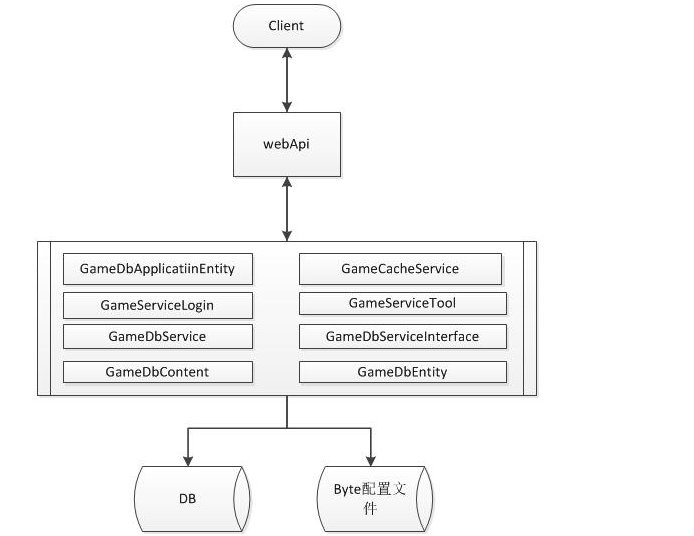
\includegraphics[width=.9\linewidth]{./pic/server_20230103_220701.png}
\begin{itemize}
\item 总结出来的缺点如下:
\end{itemize}

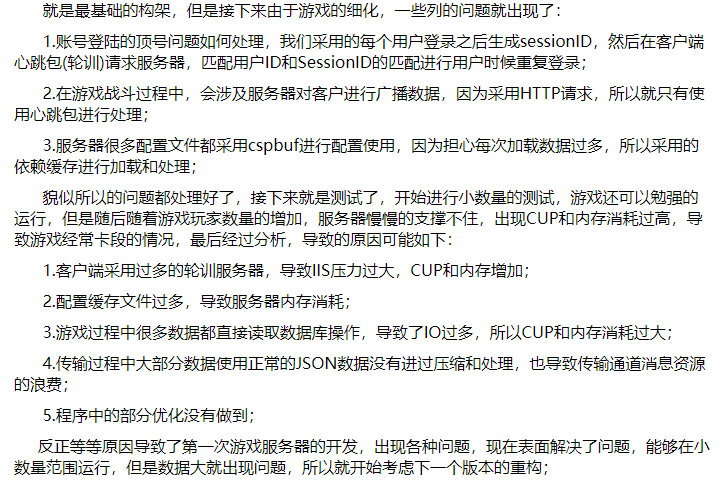
\includegraphics[width=.9\linewidth]{./pic/server_20230103_220110.png}
\begin{itemize}
\item 主要的缺点包括:
\begin{itemize}
\item 客户端心跳包:极其影响客户端与服务商性能。因为不停地周期性遍历,就不能只有注册和发生变化的时候通知一下,而不是遍历无数次吗?
\item 数据库的选择
\item 现极简小例子中涉及了将一对一同步服务器同客户端连接,重构为一服务器对10000客户端,但OOD/OOP的设计,异步调用与回调的写法,封装等,有极大的提升和优化空间(\textbf{前提是:自已能够慢慢把别人点到为止,缺失了狠多源码的讲解文的异步逻辑给真正补全,先能够异步运行起来})
\end{itemize}
\item 想要参考的比较优秀的服务端框架目前主要想参考三个:
\begin{itemize}
\item GeekServer: 对目前的我来说,仍然是读源码读得半知半解
\item ET框架
\item 和先前比较有特色的 SparkServer \url{https://github.com/Manistein/SparkServer}
\begin{itemize}
\item 主要设计思路:\url{http://manistein.club/post/server/csharp/csharp\%E6\%9C\%8D\%E5\%8A\%A1\%E7\%AB\%AF\%E6\%A1\%86\%E6\%9E\%B6\%E8\%AE\%BE\%E8\%AE\%A1\%E4\%B8\%8E\%E5\%AE\%9E\%E7\%8E\%B0/}
\end{itemize}
\end{itemize}
\item 远程服务器:是本地服务器放在网络上的某个存储和具备服务器条件的环境中运行起来,配备一个网址
\begin{itemize}
\item 服务器的网址是在哪里配置的?又翻了一遍,好像是没有看见: app\_config.json
\end{itemize}
\item (现例子源码中存在大量的游戏逻辑相关的更新,和游戏服务器服务器端本身的热更新,我的并不需要这些,我的游戏服务器甚至可以是个静态的?所以我的可以狠简单,简单到只是一个管理游戏资源包的服务器,加用户登录帐户管理,加个最基本的数据库先)
\item 数据库: 我的服务器主要是放资源包,配备资源包的版本信息,方便服务器与客户端各资源包的更新比对.
\begin{itemize}
\item 关于热更新资源包:要不要数据库呢,不要放哪里?
\item 关于用户的帐户管理:要不要数据库呢,不要怎么管理与存储?
\item 所以还是需要一个数据库的,哪怕是奇烂无比的,先用一个别人相当于是点到为止的最为基本的MySQL之类的数据库(狠怪异)?
\item 把自已项目中关于热更新资源包的源码再读和理解得透彻一些
\end{itemize}
\item 游戏服务器与普通文件服务器的区别:
\begin{itemize}
\item 文件服只需要上传下载或是浏览文件就可以了==> 简单的文件服还是满足不了游戏服的需要
\item 游戏服:尤其是自已游戏资源包的服务器,需要MD5 hash等比对文件是否发生了变化,里面还有相当一部分的逻辑是需要处理的。另登录服。。。。。
\end{itemize}
\end{itemize}
% Emacs 27.2 (Org mode 8.2.7c)
\end{document}